\subsection{Analytic 2x2}








\begin{center}
\label{tab:states-2x2}
\captionof{table}{This shows the different microstates that is possible for a 2x2 spinmatrix. It also states the energy and magnetic moment for each microstate.}
\begin{tabularx}{\textwidth}{c c c X c c c}
    \hline 
    \hline 
        State & Energy & Magnetic moment && State & Energy & Magnetic moment \\ 
    \hline
        \tilstand{1}{1}{1}{1} & -8J & 4 && \tilstand{0}{0}{0}{0} & -8J & -4 \\ \\
        
        \tilstand{0}{1}{1}{1} & 0J & 2 && \tilstand{1}{0}{0}{0} & 0J & -2 \\ \\
        \tilstand{1}{0}{1}{1} & 0J & 2 && \tilstand{0}{1}{0}{0} & 0J & -2 \\ \\
        \tilstand{1}{1}{0}{1} & 0J & 2 && \tilstand{0}{0}{1}{0} & 0J & -2 \\ \\
        \tilstand{1}{1}{1}{0} & 0J & 2 && \tilstand{0}{0}{0}{1} & 0J & -2 \\ \\

        \tilstand{0}{0}{1}{1} & 0J & 0 && \tilstand{1}{1}{0}{0} & 0J & 0 \\ \\ 
        \tilstand{0}{1}{0}{1} & 0J & 0 && \tilstand{1}{0}{1}{0} & 0J & 0 \\ \\
        \tilstand{1}{0}{0}{1} & 8J & 0 && \tilstand{0}{1}{1}{0} & 8J & 0 \\ \\
    \hline
\end{tabularx}
\end{center}



\begin{center}
\label{tab:states-2x2-summary}
\captionof{table}{The table shows a summary from table \ref{tab:states-2x2}. }
\begin{tabularx}{\textwidth}{c X c X c X c}
    \hline 
    \hline 
        Number of $\color{red}{\uparrow}$ && Multiplicity && Energy && Magnetic moment \\ 
    \hline
        4   &&      1      &&      -8J     &&       4       \\  
        3   &&      4      &&      0J      &&       2       \\
        2   &&      2      &&      8J      &&       0       \\
        2   &&      4      &&      0J      &&       0       \\
        1   &&      4      &&      0J      &&       -2      \\
        0   &&      1      &&      -8J     &&       -4      \\
    \hline
\end{tabularx}
\end{center}

\pagebreak
\subsection{example}

\begin{figure}[H]
    \centering
    \begin{subfigure}{0.5\textwidth}
        \centering
        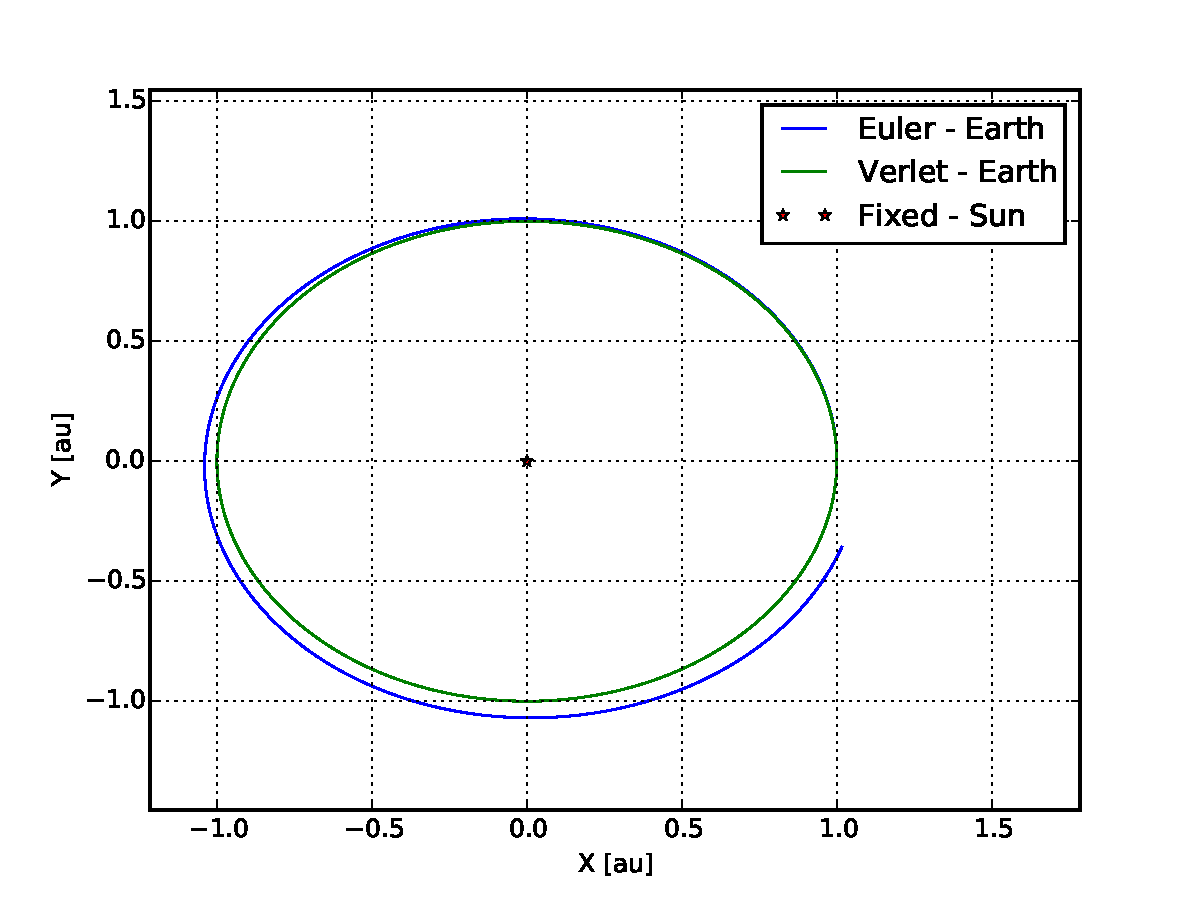
\includegraphics[width=\linewidth]{result/bilder/earth-sun.pdf}
    	\caption{}
    \end{subfigure}%
    ~ 
    \begin{subfigure}{0.5\textwidth}
        \centering
        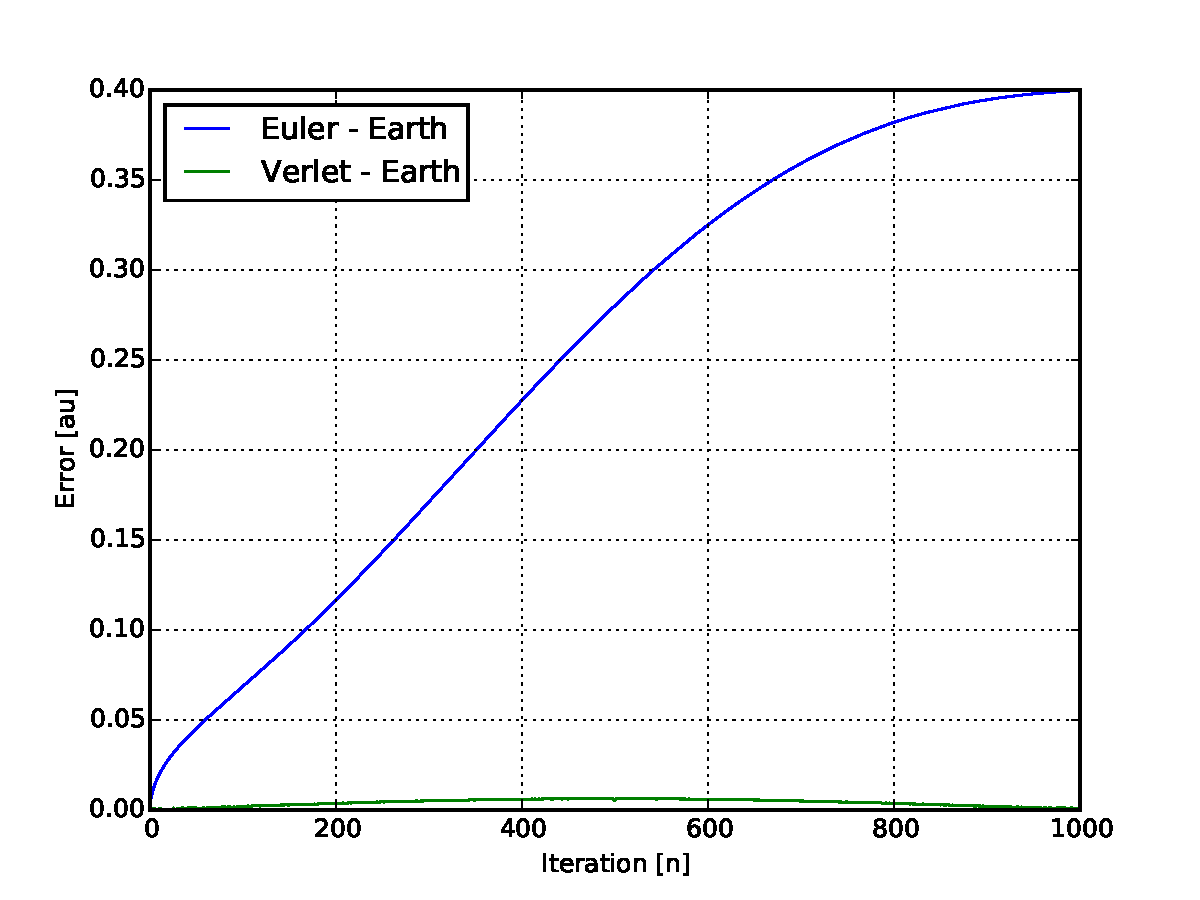
\includegraphics[width=\linewidth]{result/bilder/earth-sun-error.pdf}
        \caption{}
    \end{subfigure}
    \caption{a) shows the orbit of earth around the sun. The intial velocity is set to $2\pi$ in y direction and the start position to 1 au in x direction. b) shows how the error develops. The intial values should give a perfect circular motion. So the error is calculated by $r_i - r_{0}$. It is apparent that the Verlet-Velocity method is a better approximation. This simulation was with 1000 points with the end time of 1 year. Both simulations was produced by \href{https://github.com/erikfsk/Project-3/tree/master/Project3/earth-sun-standard-results}{\textcolor{blue}{plot\_earth\_sun.py}}}
    \label{fig:earth-sun}
\end{figure}
